% Created 2019-09-27 Fri 16:10
% Intended LaTeX compiler: pdflatex
\documentclass[11pt]{article}
\usepackage[utf8]{inputenc}
\usepackage[T1]{fontenc}
\usepackage{graphicx}
\usepackage{grffile}
\usepackage{longtable}
\usepackage{wrapfig}
\usepackage{rotating}
\usepackage[normalem]{ulem}
\usepackage{amsmath}
\usepackage{textcomp}
\usepackage{amssymb}
\usepackage{capt-of}
\usepackage{hyperref}
\author{Trey Merkley}
\date{}
\title{Fun With Frontends in Python}
\hypersetup{
 pdfauthor={Trey Merkley},
 pdftitle={Fun With Frontends in Python},
 pdfkeywords={},
 pdfsubject={},
 pdfcreator={Emacs 26.3 (Org mode 9.2.6)},
 pdflang={English}}
\begin{document}

\maketitle
\tableofcontents

\section{Python}
\label{sec:orge3b45a9}
\begin{itemize}
\item simple
\item powerful
\item usually on the backend
\end{itemize}

\#+BEGIN\textsubscript{NOTES}
Python is a language that's been used for years as a way to make complex logic feel simple. It is simple and powerful. However, its life has been dominated as being the behind-the-scenes logic supporting applications like DevOps and data science, but not on the frontend, which is a shame, because it's a great language for quickly producing robust front ends the envy of Winforms.
\#+END NOTES

\section{Qt}
\label{sec:org9633a5f}
\begin{itemize}
\item object-oriented
\item portable
\item mature
\end{itemize}

\begin{notes}
How do you pull off a pure Python frontend? With the graphical framework Qt. Qt is a GUI framework written in C++ and ported to many languages, Python among them. It's easy, object oriented, and portable to every major operating system: Windows, Mac, Linux, iOS, and Android. Additionally, it was first released in 1995 and has been actively developed by multiple organizations, making it one of the most stable GUI frameworks out there.
\end{notes}

\section{Benefits}
\label{sec:orgec5ce84}
\begin{itemize}
\item pure code
\item easy
\item well documented
\end{itemize}

\begin{notes}
So why would you want to do this, what are the benefits of writing a GUI in Python? There are some pretty great benefits to me, in addition to the above. When I was in school, all GUIs were made in Winforms using Visual Studio, and as a Linux user, this irked me to no end because, not only could I not develop and run anything I wrote on my own machine, because it was my first time developing software it really bothered me that I didn't understand the infrastructure of .NET and Winforms to understand how the graphical editor made GUIs and how to code I wrote communicated with it.

To me, Qt is a much more clear in showing the logic of how what you write all works together. You write all of the GUI code yourself (until you figure out a snippet system that works for you), and then you tie the logic to it by hand. You know where everything is at all times, and since if you're writing your frontend in Python you're almost certainly writing your logic in Python, and having all of your code in one language and having all of it hooked together by hand makes debugging much easier.

Python is easy, and using Qt is almost easier. It is intuitive for beginners and can work as an easy prototyping framework for more experienced developers.

Finally, Qt and Python implementations of Qt are \emph{very} popular, and as a result, there's a lot of information out there for how to use it. Rather than having to use only Qt's documentation, there are guides all over on how to do this stuff, and there's a great community built around developing frontends with Python.
\end{notes}

\section{Caveats}
\label{sec:orgb5caa53}
\begin{itemize}
\item Python is slower
\item Packages require work to manage
\item PyQt5 vs PySide2
\end{itemize}

\begin{notes}
So what are the caveats? Well, because Python is interpreted, it is going to be technically slower than, say C++ or C\#. However, it should not be noticeable to the average user, and you should only really need to do something else if your project grows to the size that maintaining the frontend in Python doesn't make sense, like trying to glue your Python to a C\# backend. However, if you notice that your application is stealing more than its fair share of CPU cycles and seems to be causing problems for users, it might be time to port.

Python is for the most part pretty good at package management. Unfortunately, operating systems are not, and many operating systems will install global Python files rather than letting you do it on a per application basis. As a result, you should be prepared to set up virtual environments and other isolation systems when shipping your apps to ensure they run without any unexpected problems.

Finally, there is the hairy issue of PyQt5 vs PySide2. In the long and varied history of Python and Qt integration, there are actually two packages that provide Qt for Python: PyQt5 and PySide2. Bizarrely, PyQt5 is produced by a third-party software firm called Riverbank Computing, while PySide2 is developed directly by the Qt Company. I have personally run into problems using PyQt5 that I haven't run into using PySide2. However, you try whichever you want, they both have the same libraries with the same names and the same modules, so you can drop in one for the other without having to change any of your logic, only your import statement.

So now let's look at some code.
\end{notes}

\section{Example}
\label{sec:orgf3671bc}
\begin{verbatim}
#! /usr/bin/python3 # <- Remember Python 2.7 retires in a few months

import sys # <- gets all of the system functions
from PySide2.QtWidgets import (QApplication, # <- the basic application
                               QLabel, # <- your standard labels
                               QWidget, # <- individual components of your app
                               QVBoxLayout) # <- container to tie everything together

app = QApplication(sys.argv)# <- Sets up the app and passes all command line arguments to it
window = QWidget()
layout = QVBoxLayout()
label = QLabel("<font size=40> Hello Techlahoma! </font>") # <- Has HTML style tagging
layout.addWidget(label)
window.setLayout(layout)
window.setWindowTitle("Hello Techlahoma!")
window.show()
app.exec_()
\end{verbatim}

\begin{notes}
This is the complete code of a really simple application using PySide2. We're just going to walk through this starting at the top with the shebang. Remember: Python 2.7 is about to be retired, so the time to convert your code, if written using 2.7 syntax, is now. We have to import the system module for Qt to function correctly. You have your base application, your standard label. Now Qt works by having everything individual item in your interface as a widget, including the base window itself, so we import QWidget to act as the main frame for everything to go into. Additionally, if you were to add stuff to this frame without telling Qt how it's supposed to look, it'd come out pretty weird, so we also bring in the VBoxLayout to make sure everything looks alright.

First we create the application itself. Then we make the window for the application, and the layout of that window. We also make a label. The nice thing is that QLabel will accept inline CSS style parameters, so you can set the font size and color the way you would if you were making a small web application.

From there, you add the label to the layout, and then you add the layout to the widget, set the window title so it's all pretty, and from there you create the window and run the app. When you do that you get a window that looks roughly like this:
\end{notes}

\subsection{\#+caption: A simple window in Qt}
\label{sec:org566ccf3}
\begin{center}
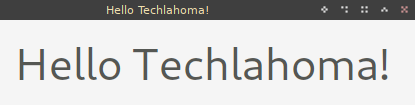
\includegraphics[width=.9\linewidth]{Screenshot_2019-09-26_16-17-12.png}
\end{center}

\begin{notes}
It's important to note that Qt uses whatever theme you have installed on your machine for its appearance, so this is what it looks like on my work laptop, but on a Windows or Mac machine it would look like a standard graphical application.
\end{notes}

\section{Getting Started}
\label{sec:orgab52b5b}
\begin{itemize}
\item \texttt{python -m pip install PySide2 -{}-user}
\item \url{https://doc.qt.io/qtforpython/tutorials/}
\item DuckDuckGo or Ecosia
\end{itemize}

\begin{notes}
So I'm not going to walk you through how to get started with Python altogether, that is for another presentation that I would imagine either Techlahoma or another group has already put up. Assuming you already have Python and Pip installed, just run \texttt{python -m pip install PySide2 -{}-user} so you can ensure it's a version for you, not the global machine. From there, just start writing! Between your autocompletion and online documentation you'll be golden. The official Qt documents are a good source, but as always, DuckDuckGo is your friend in figuring everything out.
\end{notes}

\section{End}
\label{sec:orgeb4431a}
Python ❤ Qt
\begin{itemize}
\item github.com/treymerkley
\item Slack Member ID: U7V237750
\end{itemize}

\begin{notes}
In conclusion, Python is a great language to write graphical applications. If you're just getting started and want to learn how graphical applications work, or you're trying to put together a prototype, or even if you want to roll out an app you know will run everywhere, Qt in Python is a wonderful choice to get started. I was Trey Merkley, if you have any questions at all, I'm on GitHub and Gitter, and I'm in the Techlahoma Slack channel. Thanks everyone.
\end{notes}
\end{document}
